\section{Histogramas y estadísticos completos}
Periodo: enero de 1981--diciembre de 2022. Se utilizan 485 meses completos por
variable; se excluyen 19 con faltantes, sin rellenos, prorrateos ni eliminación
automática de extremos. Se conservan los ceros. Se reúnen meses de distintas
estaciones del año, no la variabilidad de un único mes calendario.

P es precipitación CHIRPS acumulada (mm/mes); Q, caudal medio (m$^3$/s);
R, lámina de escorrentía (mm/mes). Se convierte con
$R_m=(86.4/2797.19)\sum Q_d$. R no es una observación independiente de Q.
Tmin/Tmax son medias mensuales de extremos diarios MSWX y Tmedia es estimada.

La desviación estándar es muestral, con divisor $n-1$. Para percentiles se utiliza
interpolación lineal (tipo 7): ordenados los valores, $h=(n-1)p$, con índices
desde cero, interpolando entre los vecinos de $h$. Se mantienen las unidades;
no hay una conversión de unidades para percentiles. Q1, Q2 y Q3 son los
percentiles 25, 50 y 75, e IQR = Q3--Q1.

Los histogramas usan Freedman--Diaconis, amplitud teórica $2\,IQR/n^{1/3}$;
NumPy ajusta el número entero de clases al rango. Se muestran porcentajes de
meses, no densidades; las frecuencias suman 100\,\%. Se guardan bordes y conteos.
Cuando se disponga de otra fuente de lluvia, se usarán meses comunes y clases
iguales para comparar sus distribuciones.
\begin{figure}[H]\centering
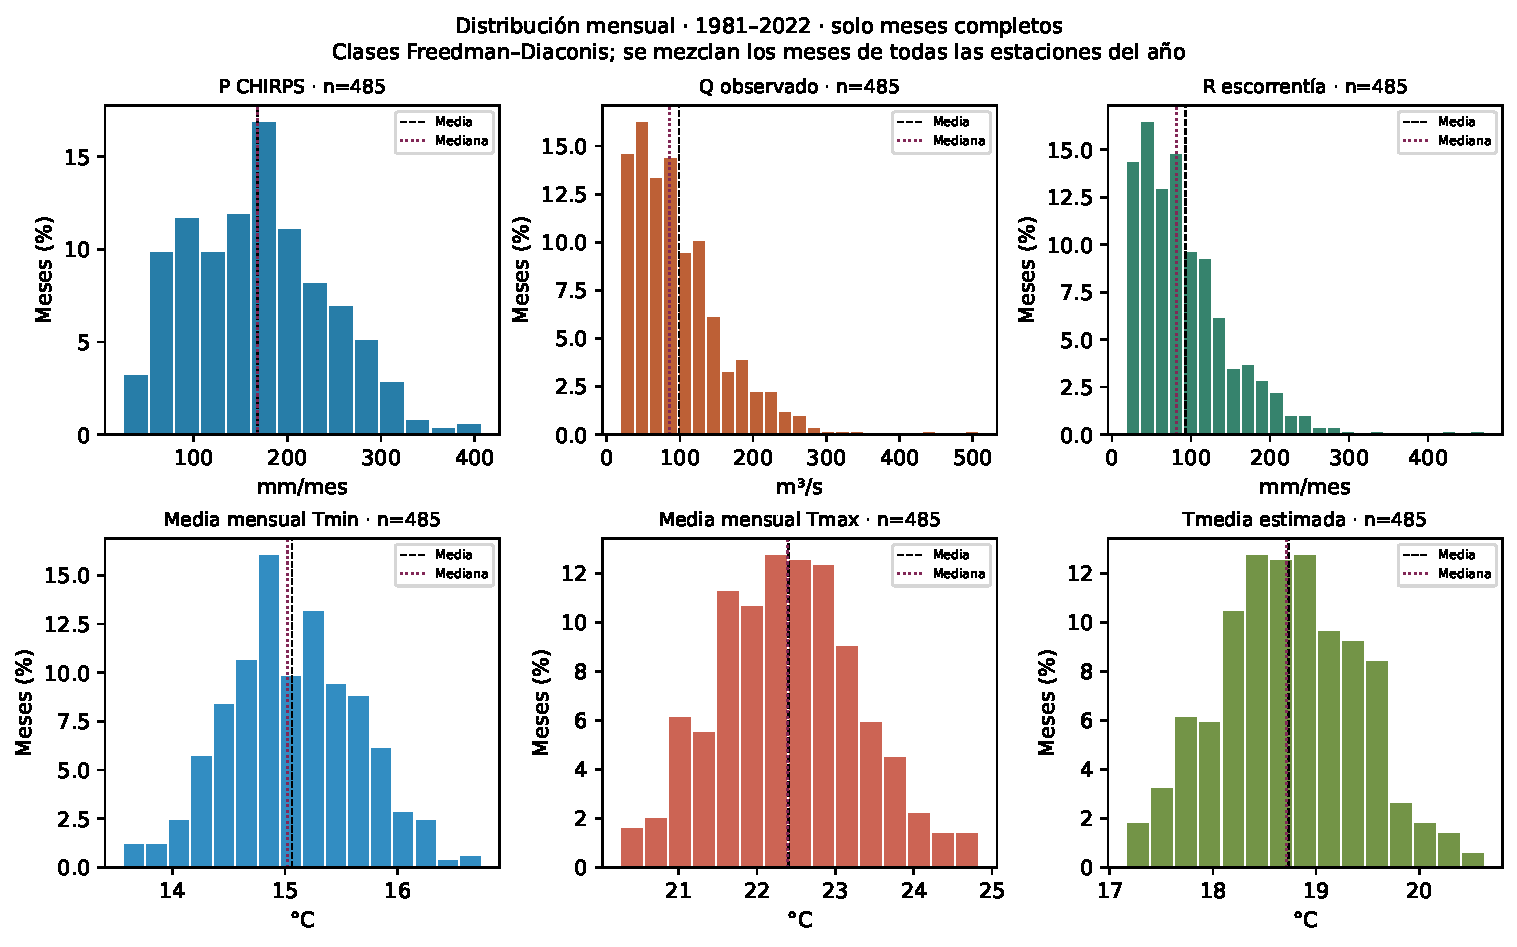
\includegraphics[width=\linewidth]{figuras/histogramas_completos.pdf}
\caption{Distribuciones de meses válidos, 1981--2022; unidades indicadas en cada panel.}
\end{figure}

\subsection{Diagramas de caja}
Se construyen diagramas de caja con los 485 meses completos entre enero de 1981 y diciembre de 2022. Los 19 meses con algún día faltante se excluyen; no se reemplazan por cero. P, Q y R no tienen meses válidos con valor cero. Para temperatura, un valor de 0~$^\circ$C se consideraría una observación válida y nunca una ausencia.

P presenta media y mediana muy próximas (168,20 y 168,47~mm), pero un rango amplio. Q y R muestran media mayor que mediana (98,70 frente a 85,55~m$^3$/s; 92,82 frente a 81,40~mm), consistente con asimetría hacia valores altos y con crecientes poco frecuentes. Los puntos fuera de 1,5 veces el IQR no se eliminan: deben revisarse en las cronologías y, cuando sea posible, contra los datos diarios y metadatos. Las cajas de temperatura son mucho más compactas que las de P, Q y R.

\begin{figure}[H]\centering
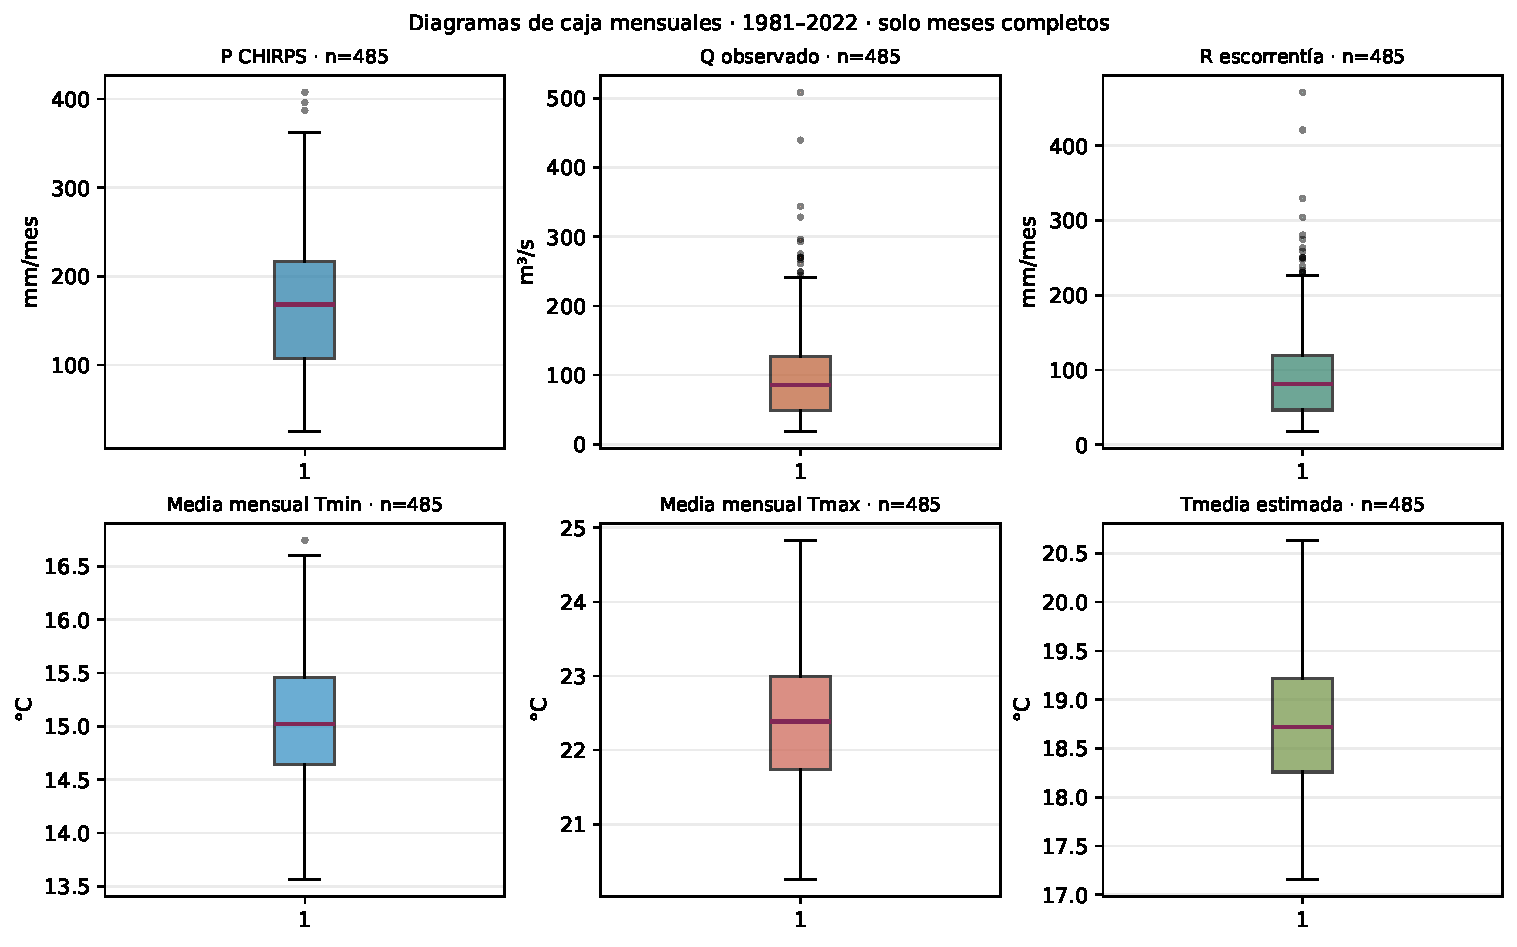
\includegraphics[width=\linewidth]{figuras/diagramas_caja.pdf}
\caption{Diagramas de caja de meses válidos. La línea central es la mediana; la caja representa Q1--Q3; los puntos son valores fuera de 1,5 IQR.}
\end{figure}

\subsection{Cuadrículas comparables: IMERG, Q, R y temperatura}
Esta sección reproduce la estructura de seis paneles de CHIRPS para permitir la comparación visual solicitada. La primera celda usa precipitación IMERG Final Run V07 y las cinco restantes usan Q, R, Tmin, Tmax y Tmedia estimada. Para que las diferencias no se deban a cobertura desigual, todas las variables se calculan sobre los mismos 285 meses completos simultáneos entre enero de 1998 y diciembre de 2022. IMERG conserva el color naranja en sus dos cuadrículas.

El bloque anterior de IMERG con 300 meses sigue siendo útil para comprobar disponibilidad total, pero estas cuadrículas comparables usan solo los 285 meses donde también existe Q. Los histogramas usan clases Freedman--Diaconis y porcentajes de meses. En las cajas, la línea central es la mediana, la caja P25--P75 y el triángulo verde la media.

\begin{figure}[H]\centering
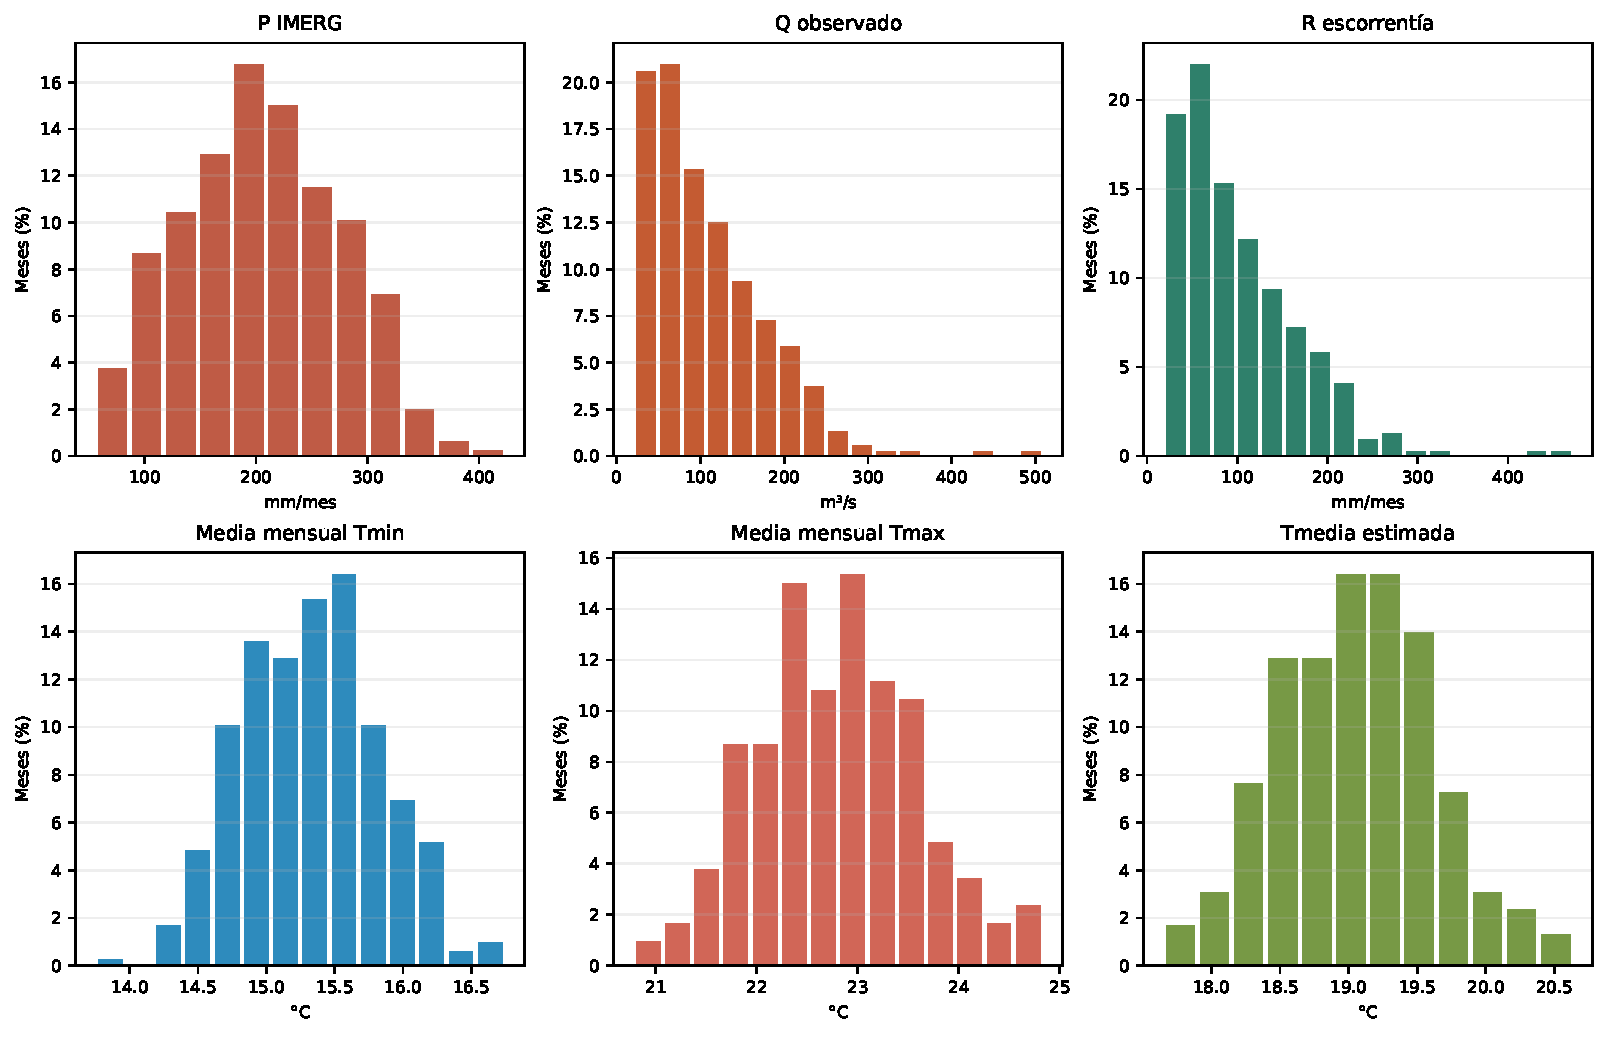
\includegraphics[width=\linewidth]{figuras/imerg_histogramas_comparables.pdf}
\caption{Histogramas comparables del periodo común: IMERG, Q, R, Tmin, Tmax y Tmedia estimada (n=285).}
\end{figure}

\begin{figure}[H]\centering
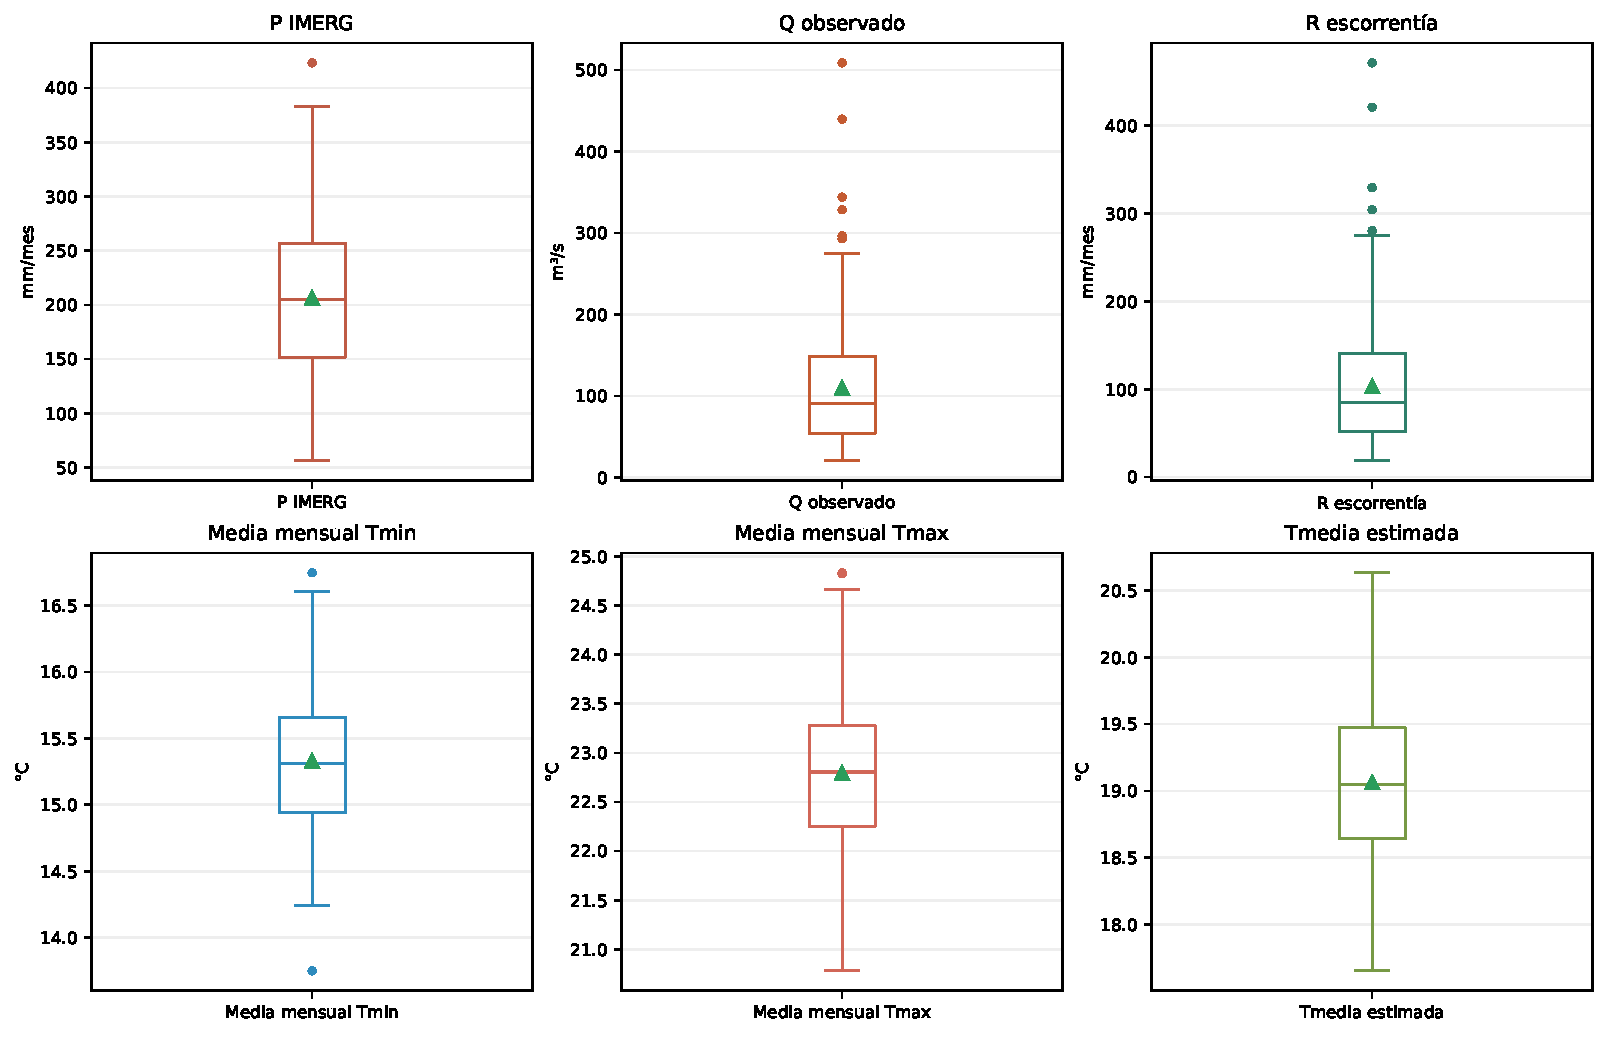
\includegraphics[width=\linewidth]{figuras/imerg_cajas_comparables.pdf}
\caption{Diagramas de caja comparables del mismo periodo común (n=285).}
\end{figure}
\subsection*{P (mm/mes), Q (m$^3$/s) y R (mm/mes)}
\begin{center}\small\begin{tabular}{lrrr}\hline
Estadístico & P & Q & R \\ \hline
Meses válidos & 485 & 485 & 485 \\
Media & 168,20 & 98,70 & 92,82 \\
Mediana & 168,47 & 85,55 & 81,40 \\
Desv. estándar & 74,54 & 64,35 & 60,63 \\
Mínimo & 24,89 & 18,37 & 17,59 \\
Máximo & 407,57 & 508,77 & 471,45 \\
Rango & 382,68 & 490,40 & 453,86 \\
Q1 (25\%) & 107,29 & 49,16 & 46,55 \\
Q2 (50\%) & 168,47 & 85,55 & 81,40 \\
Q3 (75\%) & 216,55 & 127,04 & 118,83 \\
IQR & 109,25 & 77,89 & 72,28 \\
P5 & 60,32 & 29,19 & 27,56 \\
P10 & 74,95 & 34,13 & 32,07 \\
P90 & 270,77 & 181,19 & 172,69 \\
P95 & 296,48 & 221,01 & 206,71 \\
Meses con cero & 0 & 0 & 0 \\
\hline\end{tabular}\end{center}
\subsection*{Tmin, Tmax y Tmedia estimada ($^\circ$C)}
\begin{center}\small\begin{tabular}{lrrr}\hline
Estadístico & Tmin & Tmax & Tmedia estimada \\ \hline
Meses válidos & 485 & 485 & 485 \\
Media & 15,06 & 22,40 & 18,73 \\
Mediana & 15,02 & 22,39 & 18,72 \\
Desv. estándar & 0,58 & 0,91 & 0,68 \\
Mínimo & 13,56 & 20,25 & 17,16 \\
Máximo & 16,75 & 24,83 & 20,63 \\
Rango & 3,18 & 4,58 & 3,48 \\
Q1 (25\%) & 14,65 & 21,74 & 18,26 \\
Q2 (50\%) & 15,02 & 22,39 & 18,72 \\
Q3 (75\%) & 15,46 & 23,00 & 19,22 \\
IQR & 0,81 & 1,25 & 0,96 \\
P5 & 14,17 & 20,96 & 17,61 \\
P10 & 14,34 & 21,18 & 17,81 \\
P90 & 15,81 & 23,58 & 19,60 \\
P95 & 16,05 & 23,94 & 19,84 \\
Meses con cero & 0 & 0 & 0 \\
\hline\end{tabular}\end{center}
\subsection{Precipitación in situ: existencia y alcance}
Sí existen mediciones terrestres distintas de CHIRPS. El POMCA La Vieja,
capítulo 3, tabla 3.7, documenta registros de Salento (26120160), Alcalá
(26120150), Cumbarco (26125130) y Aeropuerto El Edén (26125060).
Son mediciones puntuales; un promedio de cuenca requiere evaluar periodos,
faltantes, distribución espacial y ponderación. Fuente:
\href{https://www.cvc.gov.co/sites/default/files/Planes_y_Programas/Planes_de_Ordenacion_y_Manejo_de_Cuencas_Hidrografica/La%20Vieja%20-%20POMCA%20en%20Ajuste/Fase%20Diagnostico/3_CapituloI_Diagnostico_Clima.pdf}{POMCA La Vieja, capítulo Clima}.

Las climatologías publicadas no sustituyen una serie cronológica de 25 años.
No se han incorporado registros terrestres sin auditar: los histogramas de
precipitación de este documento corresponden a CHIRPS.
